\documentclass[11pt,aspectratio=169]{beamer}
\usepackage{amsmath,amssymb,bm,graphicx,booktabs,tikz}
\usetikzlibrary{arrows.meta,positioning}
\usetheme{default}
\setbeamertemplate{navigation symbols}{}
\setbeamertemplate{headline}{}
\setbeamertemplate{footline}{\hfill\insertframenumber/\inserttotalframenumber\hspace{0.35cm}\vspace{0.15cm}}
\setbeamertemplate{frametitle}{\vspace{0.25cm}\insertframetitle\par\vspace{0.08cm}\hrule}
\setbeamercolor{normal text}{fg=black,bg=white}
\setbeamercolor{frametitle}{fg=black,bg=white}
\setbeamercolor{structure}{fg=black}
\setbeamersize{text margin left=0.7cm,text margin right=0.7cm}
\newcommand{\dd}{\,\mathrm d}
\newcommand{\Om}{\Omega}
\newcommand{\Vzero}{\mathcal V_0}
\newcommand{\Vhzero}{\mathcal V_{h,0}}
\newcommand{\Qh}{\mathcal Q_h}
\newcommand{\grad}{\nabla}
\newcommand{\norm}[2][]{\lVert#2\rVert_{#1}}
\newcommand{\seminorm}[2][]{\lvert#2\rvert_{#1}}
\graphicspath{{figures/}}
\begin{document}

\begin{frame}
\centering\vfill
{\LARGE\bfseries Residual Error Estimation and Adaptive FEM\par}
\vspace{0.4cm}
{\large Complete the estimate, then compute and refine\par}
\vfill
\end{frame}

\begin{frame}{Lecture outline}
\begin{enumerate}
\item Collect the residual and quasi-interpolation results into the error bound.
\item Compute local indicators and use them in the adaptive loop.
\item Verify the estimator for a localized solution on a square.
\item Additional example: refine near a corner on an L-shaped domain.
\end{enumerate}
Last time we constructed $\Qh$. Today we use its local approximation estimates
to complete the error bound, then use the estimator to guide refinement.
\end{frame}

\begin{frame}{Recall the problem and the error identity}
For today's examples, $k=1$ and all boundary values are zero:
\[
-\Delta u=f\ \text{in }\Om,\qquad u=0\ \text{on }\partial\Om.
\]
Use $\Vzero=H^1_0(\Om)$ and the conforming $P_1$ space $\Vhzero\subset\Vzero$,
with
\[
a(w,v)=\int_\Om\grad w\cdot\grad v\,\dd x,\quad
\ell(v)=\int_\Om fv\,\dd x,\quad \norm[a]{v}=\sqrt{a(v,v)}.
\]
Set $e=u-u_h$. Last time, subtracting the FE equation from the continuous
equation gave
\[
R(u_h;v)=\ell(v)-a(u_h,v)=a(e,v),\qquad
R(u_h;v_h)=0\quad\forall v_h\in\Vhzero.
\]
Since $\Qh e\in\Vhzero$, choosing $v=e$ and $v_h=\Qh e$ gives
\[
\boxed{\norm[a]{e}^2=R(u_h;e)-R(u_h;\Qh e)=R(u_h;e-\Qh e).}
\]
\end{frame}

\begin{frame}{Residual representation and local approximation estimates}
Write $w=e-\Qh e$. Elementwise integration by parts gave
\[
R(u_h;w)=\sum_{e'}\int_{\mathcal K_{e'}}r_{e'}w\,\dd x
+\sum_{\mathcal F\ {\rm interior}}\int_{\mathcal F}j_{\mathcal F}w\,\dd s,
\]
where $e'$ indexes elements and $e=u-u_h$ is the error:
\[
r_{e'}=f+\Delta u_h,\qquad
j_{\mathcal F}=-(\grad u_h^+\cdot\bm n^+
                         +\grad u_h^-\cdot\bm n^-).
\]
The normals point outward from the two neighboring elements.
To bound $w$, use the following local approximation estimates for $\Qh$:
\[
\norm[L^2(\mathcal K_{e'})]{w}
 \le C_Q h_{e'}\seminorm[H^1(\omega_{e'})]{e},\qquad
\norm[L^2(\mathcal F)]{w}
 \le C_Q h_{\mathcal F}^{1/2}\seminorm[H^1(\omega_{\mathcal F})]{e}.
\]
Here $h_{e'}$ is element diameter, $h_{\mathcal F}$ is edge length, and
$\omega_{e'}$, $\omega_{\mathcal F}$ are their neighboring-element patches.
The constant $C_Q$ is independent of mesh size on a shape-regular mesh family.
\end{frame}

\begin{frame}{Mesh-size weights in the residual bound}
Start with an element integral in $R(u_h;w)$, with $w=e-\Qh e$.
Cauchy--Schwarz and the preceding local estimate give
\begin{align*}
\left|\int_{\mathcal K_{e'}}r_{e'}w\,\dd x\right|
&\le \norm[L^2(\mathcal K_{e'})]{r_{e'}}
      \norm[L^2(\mathcal K_{e'})]{w}\\
&\le C_Qh_{e'}\norm[L^2(\mathcal K_{e'})]{r_{e'}}
      \seminorm[H^1(\omega_{e'})]{e}.
\end{align*}
For an interior edge, the same two steps give
\begin{align*}
\left|\int_{\mathcal F}j_{\mathcal F}w\,\dd s\right|
&\le \norm[L^2(\mathcal F)]{j_{\mathcal F}}\norm[L^2(\mathcal F)]{w}\\
&\le C_Qh_{\mathcal F}^{1/2}\norm[L^2(\mathcal F)]{j_{\mathcal F}}
      \seminorm[H^1(\omega_{\mathcal F})]{e}.
\end{align*}
These are the origins of the element weight $h_{e'}$ and edge weight
$h_{\mathcal F}^{1/2}$.
\end{frame}

\begin{frame}{Collect the estimates into the global bound}
Add the bounds on the preceding slide, using $\norm[a]{e}^2=R(u_h;w)$:
\begin{align*}
\norm[a]{e}^2\le C_Q\bigg[
&\sum_{e'}h_{e'}\norm[L^2(\mathcal K_{e'})]{r_{e'}}
                   \seminorm[H^1(\omega_{e'})]{e}\\
+&\sum_{\mathcal F\ {\rm interior}}h_{\mathcal F}^{1/2}
\norm[L^2(\mathcal F)]{j_{\mathcal F}}
                   \seminorm[H^1(\omega_{\mathcal F})]{e}\bigg]
\le C_Q\eta B.
\end{align*}
The last step is Cauchy--Schwarz over the combined list of entries, with
\begin{align*}
\eta^2&=\sum_{e'}h_{e'}^2\norm[L^2(\mathcal K_{e'})]{r_{e'}}^2
+\sum_{\mathcal F\ {\rm interior}}h_{\mathcal F}
\norm[L^2(\mathcal F)]{j_{\mathcal F}}^2,\\
B^2&=\sum_{e'}\seminorm[H^1(\omega_{e'})]{e}^2
+\sum_{\mathcal F\ {\rm interior}}\seminorm[H^1(\omega_{\mathcal F})]{e}^2.
\end{align*}
\end{frame}

\begin{frame}{Complete the reliability bound}
Start from $\norm[a]{e}^2\le C_Q\eta B$ on the preceding slide.
On a shape-regular mesh family, each gradient integral is counted in at most
$N_{\rm ov}$ patches. Since $k=1$,
\[
 B^2=\sum_{e'}\seminorm[H^1(\omega_{e'})]{e}^2
 +\sum_{\mathcal F\ {\rm interior}}\seminorm[H^1(\omega_{\mathcal F})]{e}^2
 \le N_{\rm ov}\seminorm[H^1(\Om)]{e}^2
       =N_{\rm ov}\norm[a]{e}^2.
\]
Substitute $B\le\sqrt{N_{\rm ov}}\norm[a]{e}$:
\[
\norm[a]{e}^2\le C_Q\sqrt{N_{\rm ov}}\eta\norm[a]{e}.
\]
Divide by $\norm[a]{e}$ if it is nonzero:
\[
\boxed{\norm[a]{u-u_h}\le C_{\rm rel}\eta,\qquad
 C_{\rm rel}=C_Q\sqrt{N_{\rm ov}}.}
\]
If the error is zero, the inequality holds without division.
\end{frame}

\begin{frame}{Main result: a computable residual estimator}
Assume a bounded Lipschitz domain, $f\in L^2(\Om)$, conforming shape-regular
$P_1$ meshes, the stated quasi-interpolation estimates, and exact FE assembly
and solution. Then
\[
\boxed{\norm[a]{u-u_h}\le C_{\rm rel}\eta,\qquad
\eta^2=\sum_e\eta_e^2,}
\]
where
\[
\boxed{\eta_e^2=h_e^2\norm[L^2(\mathcal K_e)]{r_e}^2
+\frac12\sum_{\substack{\mathcal F\subset\partial\mathcal K_e\\
                       \mathcal F\ {\rm interior}}}
h_{\mathcal F}\norm[L^2(\mathcal F)]{j_{\mathcal F}}^2.}
\]
Each interior edge belongs to two elements, so its total weight is
$1/2+1/2=1$. Summing the local indicators recovers the global formula above.
\[
r_e=f+\Delta u_h=f\quad\text{for }P_1\text{ triangles and }k=1.
\]
For a nonzero source, the volume contribution remains even though
$\Delta u_h=0$ inside an element.
\end{frame}

\begin{frame}{What the estimator tells us}
\textbf{Reliability:}
$\norm[a]{u-u_h}\le C_{\rm rel}\eta$ bounds the unknown energy error.
The constant is independent of mesh size, but need not equal one.

\vspace{0.25cm}
\textbf{Local indicators:} $\eta_e^2$ show which elements contribute most
to $\eta^2$. They are not exact element errors. An efficiency estimate compares
them with nearby error and unresolved variation in the data. It requires a
separate proof.

\vspace{0.25cm}
\textbf{Verification with a known solution:}
\[
E_a=\norm[a]{u_{\rm ex}-u_h},\qquad
I_{\rm eff}=\frac{\eta}{E_a}\quad(E_a>0).
\]
Effectivity is the ratio of the estimator to the actual energy error.
Our first example allows this check; the corner example does not.
\end{frame}

\begin{frame}{From the local formula to an assembled vector}
Use a discontinuous constant space, called \texttt{DG0} in FEniCSx.
Its basis function $z_e$ equals $1$ on $\mathcal K_e$ and $0$ elsewhere.
The local formula can therefore be written
\[
\eta_e^2=\int_\Om h^2r^2z_e\,\dd x+
\sum_{\mathcal F\ {\rm interior}}\int_{\mathcal F}
h_{\mathcal F}j_{\mathcal F}^2\,
\frac{z_e^++z_e^-}{2}\,\dd s.
\]
On an edge belonging to $\mathcal K_e$, the average of $z_e$ is $1/2$,
which assigns the required half contribution to each neighbor.

The notebook assembles volume and facet terms separately and adds them.
The resulting vector has one squared indicator per element.
No division by element area is needed.

\end{frame}

\begin{frame}{Marking and the adaptive loop}
Choose $0<\theta<1$. \textbf{D\"orfler marking} selects a set of elements
$\mathcal M$ such that
\[
\boxed{\sum_{\mathcal K_e\in\mathcal M}\eta_e^2
       \ge\theta\sum_e\eta_e^2.}
\]
Sort squared indicators from largest to smallest and add elements until their
sum reaches the target. The notebook uses $\theta=0.5$.
\[
\boxed{\text{solve}\ \longrightarrow\ \text{estimate}\ \longrightarrow\
       \text{mark}\ \longrightarrow\ \text{refine}}
\]
After refinement, solve the PDE again and recompute all indicators.
Neighboring elements may also be refined to maintain a conforming mesh.

An estimator tolerance $\eta\le\varepsilon_{\rm est}$ gives
$\norm[a]{u-u_h}\le C_{\rm rel}\varepsilon_{\rm est}$.
Today we use fixed cycle counts to keep the demonstration short.
\end{frame}

\begin{frame}
\centering\vfill
{\LARGE\bfseries Example 1: a localized solution\par}
\vspace{0.35cm}
{\large Verify the estimator, then compare adaptive and uniform refinement.\par}
\vfill
\end{frame}

\begin{frame}{A Gaussian pulse on the unit square}
Take $\Om=(0,1)^2$ and prescribe zero values on every boundary edge:
\[
-\Delta u=f\quad\text{in }\Om,\qquad u=0\quad\text{on }\partial\Om.
\]
Set $\alpha=400$, $s_i=x_i-\tfrac12$, $G_i=e^{-\alpha s_i^2}$, and
$c=e^{-\alpha/4}$. Choose the known solution
\[
\boxed{u_{\rm ex}=(G_1-c)(G_2-c)}
\]
and define the source by differentiating this expression:
\[
f(x_1,x_2)=-\Delta u_{\rm ex}(x_1,x_2).
\]
If $x_i=0$ or $1$, then $G_i=c$, so $u_{\rm ex}=0$ on the boundary.

{\small Adapted from Larson--Bengzon, \S4.9.3, Eq.~(4.130), printed p.~91:
normalized and boundary-corrected so the prescribed values hold exactly.}
\end{frame}

\begin{frame}{What to examine in the notebook}
\begin{enumerate}
\item Solve on an $8\times8$ square grid, split into 128 triangles.
\item Plot the FE solution and indicators. Which elements contribute most?
\item Mark and refine once; compute a new FE solution.
\item Repeat and compare with uniform refinement at comparable DOF counts.
\end{enumerate}
Because $u_{\rm ex}$ is known, calculate
\[
E_a=\left(\int_\Om\grad(u_{\rm ex}-u_h)\cdot
                       \grad(u_{\rm ex}-u_h)\,\dd x\right)^{1/2},
\qquad I_{\rm eff}=\eta/E_a.
\]
Use the analytic solution, not its nodal interpolant, in this error integral.
The Gaussian is not a polynomial: volume quadrature must resolve the pulse.

\href{../../../notebooks/adaptivity/residual_adaptivity.ipynb}{Open the companion notebook.}
\end{frame}

\begin{frame}{One adaptive refinement step}
\centering
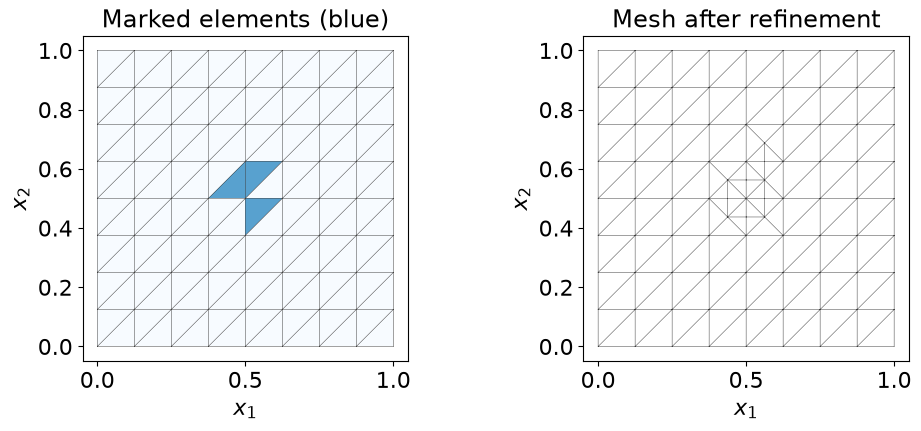
\includegraphics[width=0.94\textwidth,height=0.70\textheight,keepaspectratio]{c8_pulse_marked_refined.png}

\small Blue elements are selected from the computed indicators, not from
the known solution. The right mesh includes refinement needed for conformity.
\end{frame}

\begin{frame}{Where the mesh becomes finer}
\centering
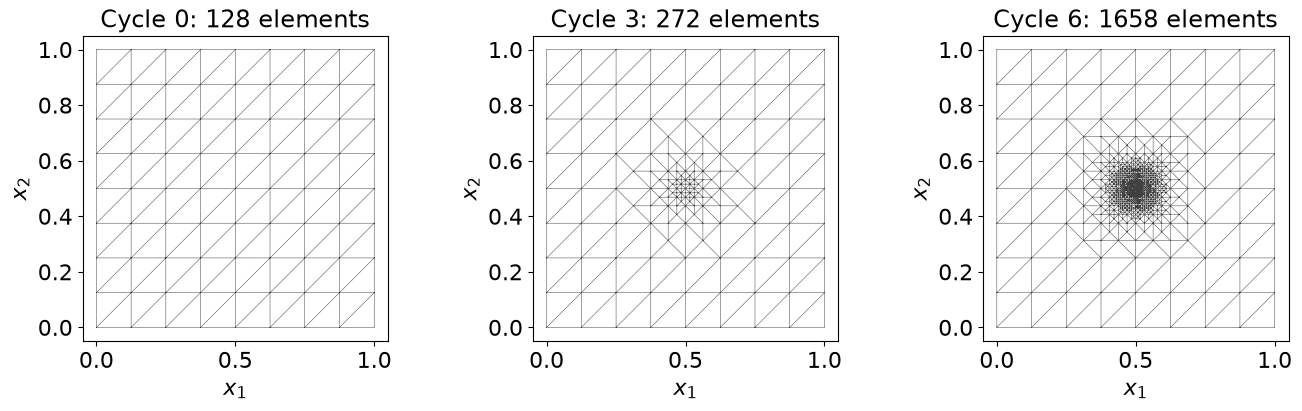
\includegraphics[width=0.98\textwidth,height=0.70\textheight,keepaspectratio]{c8_pulse_mesh_history.png}

\small The residual indicators concentrate refinement near the localized pulse.
The same solve--estimate--mark--refine operations are repeated at each cycle.
\end{frame}

\begin{frame}{Verify error reduction and estimator behavior}
\centering
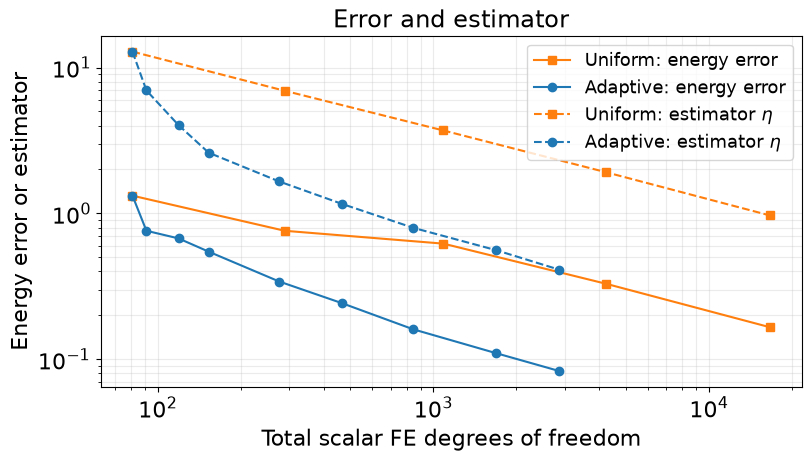
\includegraphics[width=0.98\textwidth,height=0.69\textheight,keepaspectratio]{c8_pulse_verification.png}

\small Solid curves: actual energy error. Dashed curves: estimator.
Selective refinement gives smaller errors at comparable DOF counts here.
\end{frame}

\begin{frame}{Effectivity: compare the estimator with the actual error}
\centering
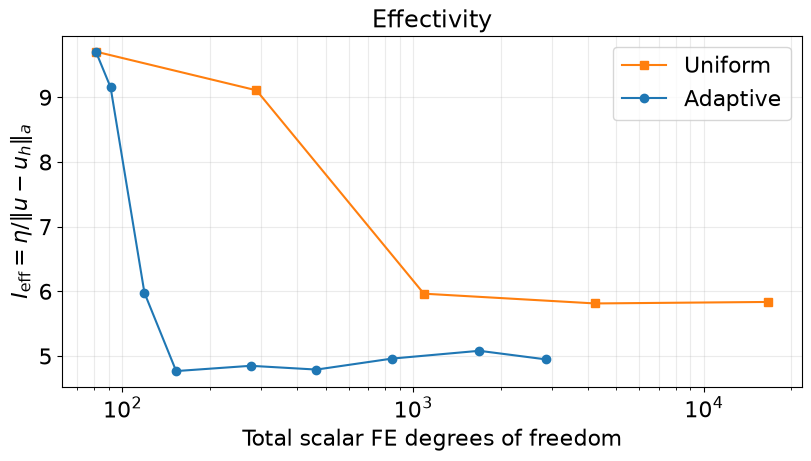
\includegraphics[width=0.94\textwidth,height=0.69\textheight,keepaspectratio]{c8_pulse_effectivity.png}

\small Effectivity is $\eta/\norm[a]{u_{\rm ex}-u_h}$.
It approaches a factor near five for the adaptive meshes, not one.
This ratio is measured here because the exact solution is known.
\end{frame}

\begin{frame}
\centering\vfill
{\LARGE\bfseries Additional example: a corner\par}
\vspace{0.35cm}
{\large Use the same estimator when the exact solution is unknown.\par}
\vfill
\end{frame}

\begin{frame}{Diffusion on the L-shaped domain}
\begin{columns}[T,onlytextwidth]
\begin{column}{0.44\textwidth}
\centering
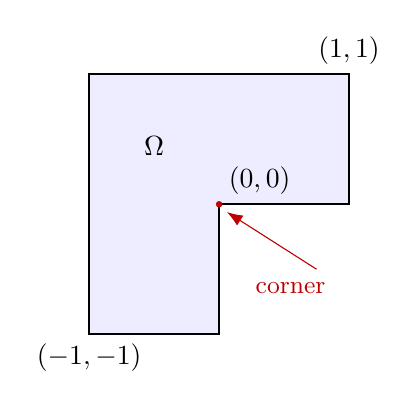
\begin{tikzpicture}[scale=1.65]
\draw[thick,fill=blue!7] (-1,-1)--(0,-1)--(0,0)--(1,0)--(1,1)--(-1,1)--cycle;
\fill[red!75!black] (0,0) circle[radius=0.025];
\draw[-{Latex[length=2mm]},red!75!black] (0.75,-0.5)--(0.06,-0.06);
\node[red!75!black,font=\small,anchor=north] at (0.55,-0.53) {corner};
\node at (-0.5,0.45) {$\Om$};
\node[below] at (-1,-1) {$(-1,-1)$};
\node[above] at (1,1) {$(1,1)$};
\node[above right] at (0,0) {$(0,0)$};
\end{tikzpicture}
\end{column}
\begin{column}{0.53\textwidth}
Remove the lower-right quadrant:
\[
\Om=\{(x_1,x_2)\in(-1,1)^2:
x_1<0\ \text{or}\ x_2>0\}.
\]
Solve
\[
\left\{\begin{aligned}
-\Delta u&=1&&\text{in }\Om,\\
u&=0&&\text{on }\partial\Om.
\end{aligned}\right.
\]
The same estimator applies, now with $r_e=1$.
The exact solution is unknown, so we cannot compute effectivity here.
\end{column}
\end{columns}
\vspace{0.12cm}
{\footnotesize Arnold, Chapter 4, \S9.5, printed p.~74 (PDF p.~78).}
\end{frame}

\begin{frame}{Refinement near the corner}
\centering
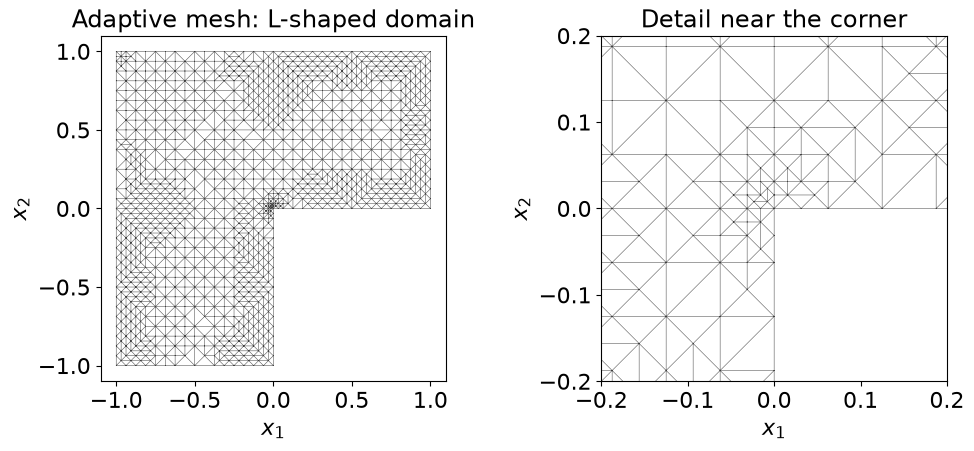
\includegraphics[width=0.94\textwidth,height=0.68\textheight,keepaspectratio]{c8_corner_mesh.png}

\small The reentrant corner reduces regularity; the solution is not in
$H^2(\Om)$. Reliability uses the $H^1$ error, not an $H^2$ assumption.
The indicators produce smaller elements near the corner without a
distance-based refinement rule.
\end{frame}

\begin{frame}{Summary}
\begin{itemize}
\item The Gaussian example compares $\eta$ with a measured energy error.
The actual errors show the benefit of local refinement for this localized
solution.
\item The corner example shows where the same indicators place resolution
when the exact solution is unknown. Its estimator values are not exact errors.
\item Both examples retain volume and interior-edge terms and use the same
marking and refinement procedure.
\end{itemize}
\[
\boxed{\norm[a]{u-u_h}\le C_{\rm rel}\eta,\qquad
       \eta^2=\sum_e\eta_e^2.}
\]
\end{frame}

\begin{frame}{References and further details}
\begin{itemize}
\item Course book, Chapter 8, Sections 8.4--8.5: residual estimator and reliability.
\item Larson--Bengzon, 2010 notes, \S4.9.1, Theorem 4.7,
Eqs.~(4.115)--(4.116), printed p.~88; \S4.9.3, printed pp.~90--92:
adaptive examples, including the Gaussian pulse on p.~91.
\item Arnold, \emph{Lecture Notes on Numerical Analysis of Partial
Differential Equations}, Chapter 4, \S\S9.3--9.5, printed pp.~71--76:
residual estimates, marking, and the L-shaped example.
\end{itemize}
The supporting reading decks retain the longer derivations and calculations.
\end{frame}

\end{document}
